\subsection{Person 5 – SUS 87.5}  
\textbf{Zur Person:}\\
IT-Projektmanager, 59 Jahre alt  

\textbf{Beobachtung:}  
\begin{enumerate}
    \item Zeichnen Sie frei für etwa 2 Minuten.
    \begin{itemize}
        \item Suchte vordefinierte Formen.
        \item Frage: Wiso gümmelt es den Hintergrund?.
        \item Bug: Stift-Menü geöffnet → keine direkte Anpassung möglich; Stift erscheint immer zuerst blau.
    \end{itemize}

    \item Löschen Sie Ihre Zeichnung vollständig.
    \begin{itemize}
        \item Kein Problem.
    \end{itemize}

    \item Laden Sie die PDF-Datei mit dem Grundriss hoch.
    \begin{itemize}
        \item Nur ein Button vorhanden, unklar, ob für Öffnen oder Exportieren.
    \end{itemize}

    \item Ändern Sie die Stiftfarbe auf Rot.
    \begin{itemize}
        \item Kein Problem, bereits vorher herausgefunden.
        \item Leichte Offsets beim Zeichnen.
    \end{itemize}

    \item Suchen Sie \texttt{BEDROOM3} und zeichnen Sie einen Tisch links vom Bett.
    \begin{itemize}
        \item Kein Problem.
    \end{itemize}

    \item Radieren Sie den Tisch und zeichnen Sie ihn rechts vom Bett.
    \begin{itemize}
        \item Verschiebe-Offset-Problem; Zoom nötig.
        \item Selektion- und Verschiebe-Tool wäre hilfreich.
        \item Wunsch nach Form-Katalog (Tische, Stühle etc.).
    \end{itemize}

    \item Zeichnen Sie die Abmessungen 1\,m $\times$ 1\,m und schreiben Sie «table» hinein.
    \begin{itemize}
        \item Schreiben auf Tisch: Schriftgrösse nicht optimal, zu klein + Offset beim genauen Einzeichnen.
    \end{itemize}

    \item Speichern Sie den Plan auf Ihrem Laptop.
    \begin{itemize}
        \item Kein Problem.
    \end{itemize}
\end{enumerate}

\clearpage

\textbf{SUS-Antworten (Bild):}
\begin{center}
    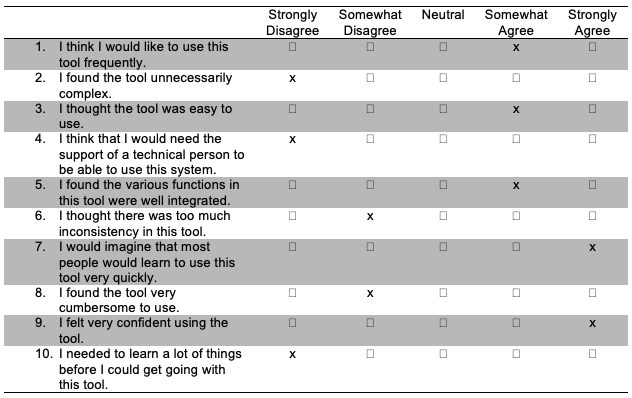
\includegraphics[width=0.95\textwidth]{graphics/sus_person5.png}
\end{center}

\textbf{Follow-up:}  
\begin{enumerate}
    \item \textbf{Was hat Ihnen am Tool am besten gefallen?}
    \begin{itemize}
        \item Grosse Stifte auf dem Tisch nutzen, Möglichkeit für Team-Planungsdiskussionen.
    \end{itemize}

    \item \textbf{Gab es etwas, das verwirrend oder schwierig zu bedienen war?}
    \begin{itemize}
        \item Offsets beim Zeichnen (vor allem beim Zoomen).  
        \item Hintergrund „gümmelet“ → suboptimal zum Arbeiten.
    \end{itemize}

    \item \textbf{Fehlt etwas, das Sie erwartet oder gerne gehabt hätten? / Verbesserungsvorschläge}
    \begin{itemize}
        \item Form-Katalog (Stühle, Tische, etc.)  
        \item Bereiche/Objekte verschieben und kopieren  
        \item Druckfunktion vom oberen Button integrieren  
        \item Mit einem grösseren Tisch sollte das Präzisionsproblem weniger auffallen
    \end{itemize}
\end{enumerate}

\clearpage
